%%%%%%%%%%%%%%%%%%%%%%%%%%%%%%%%%%%%%%%%%%%%%
%第5章

\chapter{実験} % 章の見出し
本章では,以下の4点に関して実際に文書検索精度を比較することで,
どのように精度が変化するかを調査・分析する.
\begin{itemize}
    \item TF-IDFにおけるTFの正規化                
    \item 単語の意味的情報の加味                  
    \item 部分文書検索における文書全体の情報の加味
    \item 音声認識誤りの棄却                      
\end{itemize}

\section{実験条件}
\begin{table}[htbp]
    \begin{center}
        \caption{実験条件}
        \begin{tabular}{|c|c|}
            \hline
            全体文書数 & 98文書 \\ \hline
            部分文書数 & 2807文書 \\ \hline
            クエリ数 & 35個 \\ \hline
            word2vec学習コーパス & Web文書 述べ語数14億語 \\ \hline
            PMI学習コーパス & 日本語話し言葉コーパス CSJ \\ \hline
        \end{tabular}
        \label{t_condition}
    \end{center}
\end{table}
実験は,NTCIR11 SpokenQuery\&Doc Formal-run の SQSCR SGS Retrieval条件で行った.
実験条件を表\ref{t_condition}に示す.
特に指定しない限り,以下の実験ではクエリ・文書共に音声を人手で書き起こした条件で行った.
評価尺度にはMAP値を用いた.これはクエリ毎の平均適合率AP値の平均である.クエリ$q$に対するAP値$AP(q)$は式(\ref{eq_ap})で計算される.
\begin{equation}
    AP(q) = \frac{1}{N} \sum^N_{i=1} \frac{i}{rank(i)}    \label{eq_ap}
\end{equation}
ここで$N$はクエリ$q$に対する正解文書の数,$rank(i)$はクエリ$q$の$i$番目の正解文書が,文書検索によって付けられた順位である.
AP値,MAPは共に[0, 1]の値をとる.

\section{実験結果}
\begin{table}[htbp]
    \begin{center}
        \caption{書き起こしを用いた文書検索精度}
        \begin{tabular}{|c|l|}
            \hline
            & MAP \\ \hline
            TF-IDF & 0.1629 \\ \hline \hline
            log\_TF-IDF & 0.1630 \\ \hline
            BM25 & 0.1880 \\ \hline
            word2vec & 0.1057 \\ \hline
            global & 0.2745 \\ \hline
        \end{tabular}
        \label{t_text}
    \end{center}
\end{table}
実験結果を表\ref{t_text}に示す.なお表中のword2vecはword2vecを用いた文書検索法であり,
globalはTF-IDFによる文書検索の結果に,文書全体の情報を加味したものである.
なお,$\alpha$は0.1刻みで0.1から0.9まで変化させた.

\subsection{TF-IDFにおけるTFの正規化}
\begin{figure}
    \centering
    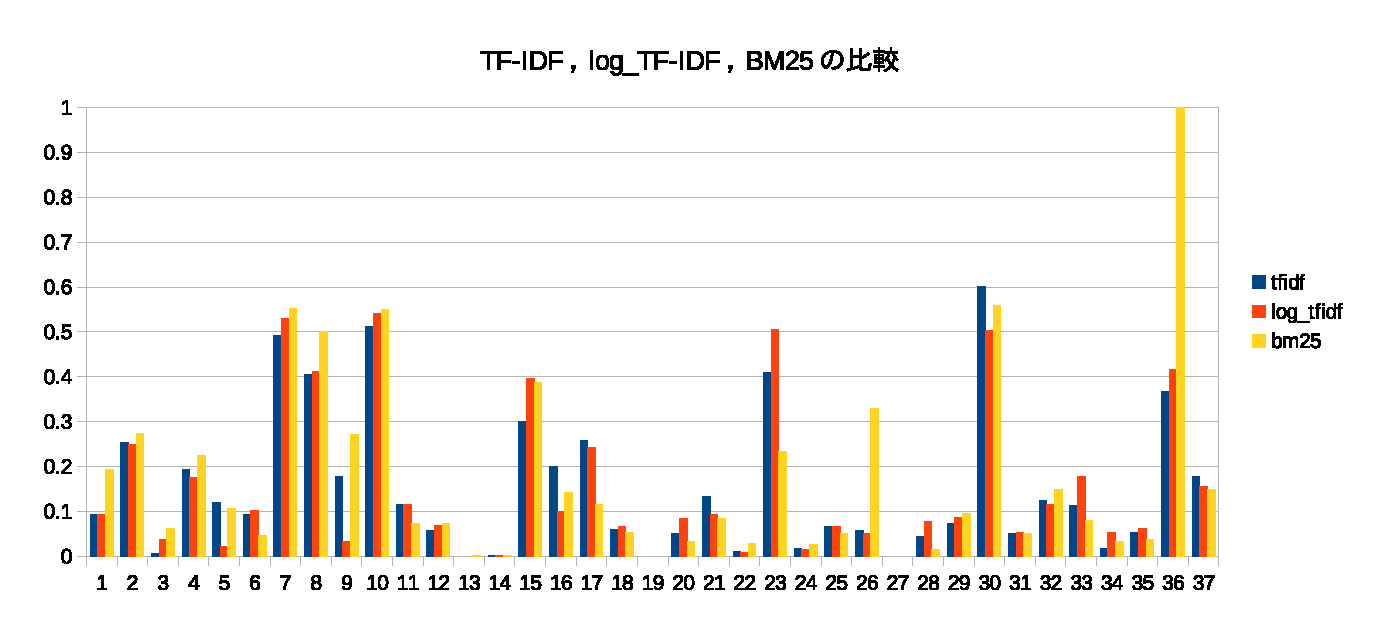
\includegraphics[width=7cm]{./graph/TFIDF_log_BM25.eps}
    \caption{TF-IDF, log\_TF-IDF, BM25のクエリ別検索精度}
    \label{fig_tf_log_BM25}
\end{figure}
表\ref{t_text}においてTF-IDFとlog\_TF-IDFのMAP値を比較すると,文書検索においてほぼ同等の性能があることがわかる.
ただし図\ref{fig_tf_log_BM25}から,log\_TF-IDFはTF-IDFより,正解文書が短いクエリに対して精度が良く,正解文書が長いクエリについてはTF-IDFより精度が下がる傾向があることがわかる.
一方でBM25はlog\_TF-IDFと同様の傾向があるが,一部のクエリにおいてTF-IDFの精度を大きく改善している.
これらのことから,TF-IDFにおいて文書長に応じてTFを正規化することにより,文書検索精度を向上させることができると考えられる.

\subsection{単語の意味的情報の加味}
\begin{figure}
    \centering
    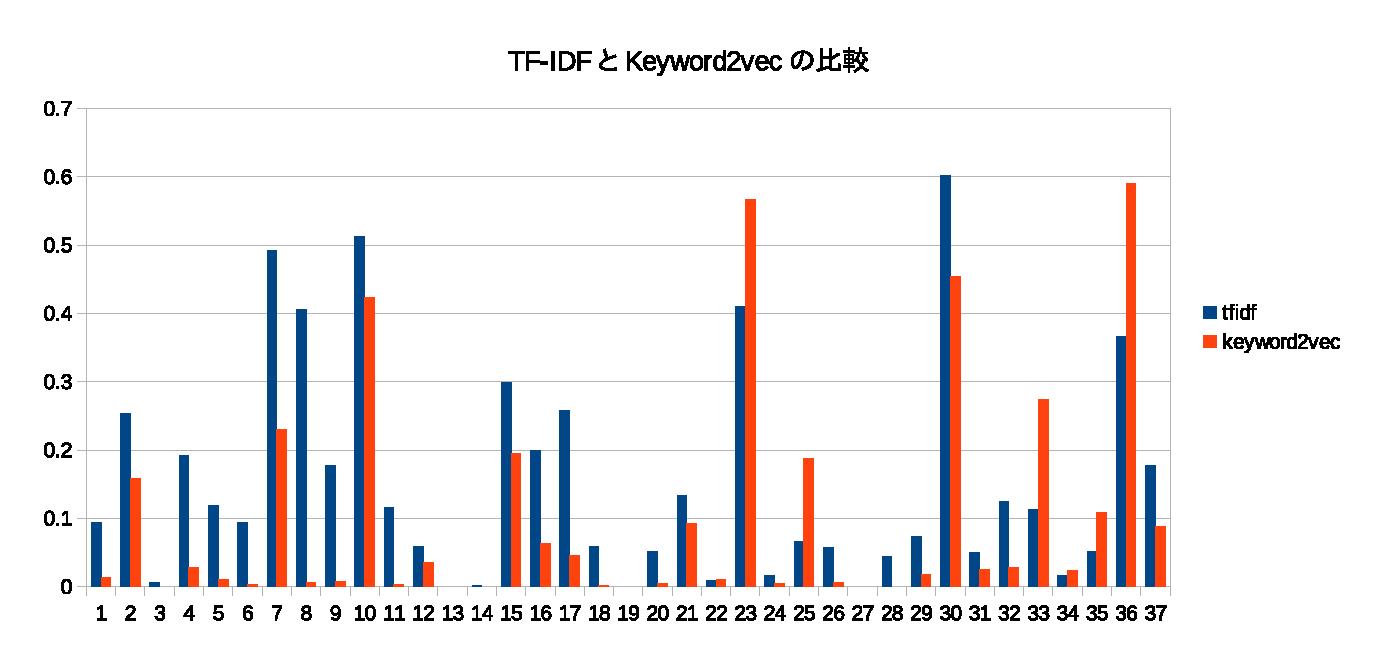
\includegraphics[width=7cm]{./graph/TFIDF_keyword2vec.eps}
    \caption{TF-IDF, log\_TF-IDF, BM25のクエリ別検索精度}
    \label{fig_tf_word2vec}
\end{figure}
表\ref{t_text}においてTF-IDFとword2vecのMAP値を比較すると,単語の意味的情報を考慮しないTF-IDFの方が優れた検索性能があることが分かる.
一方で図\ref{fig_tf_word2vec}から,word2vecは全体の精度では劣るが,一部のクエリにおいてTF-IDFを大きく上回る検索精度を示していることが分かる.
よって\ref{sec_word2vec}節に示した検索法は,従来法との組み合わせにより検索性能を大きく向上させることが
できると考えられる.

\subsection{部分文書検索における文書全体の情報の加味}
$\alpha = 0.9$のとき,表\ref{t_text}よりMAP値が最大値0.2745となった.
これは部分文書検索において,文書全体の情報を用いることが精度向上に大きく貢献することを意味する.

\subsection{音声認識誤りの棄却}
\begin{table}[htbp]
    \begin{center}
        \caption{音声認識結果を用いた文書検索精度}
        \begin{tabular}{|c|l|}
            \hline
                     &   MAP   \\ \hline
            棄却無し & 0.1067 \\ \hline
            棄却あり & 0.09406 \\ \hline
        \end{tabular}
        \label{t_spoken}
    \end{center}
\end{table}
音声認識結果のクエリ・文書を用いて文書検索を行った.
表\ref{t_spoken}に結果を示す.
表\ref{t_spoken}より,誤り棄却がある場合の方が逆に精度が劣化していることが分かる.
ここで誤り単語の棄却率は,FARが0.241,FRRが0.406であった.
このことから,認識誤り単語の棄却はできるが,その一方で検索に有用な語を棄却したため,精度が劣化したことが分かる.
しかし一方で,単語$w$を認識誤り単語とする$sumPMI(w)$の閾値を変化させることで,検索精度が向上する可能性があると言える.
